\documentclass[12pt, a4paper, UTF8, fontset=windows]{ctexbook}
\usepackage{amsmath, amsthm, amssymb, amsfonts, bm, color, enumitem, fancyhdr, framed, float, geometry, graphicx, hyperref, lastpage, listings, mathrsfs, xcolor}


\linespread{1.5}
\definecolor{shadecolor}{RGB}{241, 241, 255}
\newcounter{problemname}
\newenvironment{problem}{\begin{shaded}\stepcounter{problemname}\par\noindent\textbf{Q\arabic{problemname}.}}{\end{shaded}\par}
\newenvironment{solution}{\par\noindent\textbf{Ans.}}{\par}

\geometry{left=20mm,right=20mm, top=20mm, bottom=22mm} % 页边距
\setlength{\headheight}{15pt}
\pagestyle{fancy} % 设置页脚页眉
\rhead{Assignment1} % 页眉右边
% \noindent % 取消首段缩进

\definecolor{mygreen}{rgb}{0,0.6,0}
\definecolor{mygray}{rgb}{0.5,0.5,0.5}
\definecolor{mymauve}{rgb}{0.58,0,0.82}
% 代码设置
\lstset{ 
    backgroundcolor=\color{white},      % choose the background color
    basicstyle=\footnotesize\ttfamily,  % size of fonts used for the code
    columns=fullflexible,
    tabsize=4,
    breaklines=true,               % automatic line breaking only at whitespace
    captionpos=b,                  % sets the caption-position to bottom
    commentstyle=\color{mygreen},  % comment style
    keywordstyle=\color{blue},     % keyword style
    stringstyle=\color{mymauve}\ttfamily,  % string literal style
    frame=single,
    rulesepcolor=\color{red!20!green!20!blue!20},
    language=c++,
    xleftmargin=3em,
    xrightmargin=3em
}


\begin{document}

\cfoot{\thepage\ / \pageref{LastPage}} % 页眉中间位添加内容:页码/总页码

\thispagestyle{empty}

\begin{figure}[t]
    \centering
    
\includegraphics[width=6cm]{../../src/images/logo.jpg}
\end{figure}

\vspace*{\fill}
    \begin{center}
        \Huge\textbf{Assignment1}
    \end{center}
\vspace*{\fill}

\begin{table}[b]
    \centering
    \large
    \begin{tabular}{ll}
        \textbf{Course:} & Computer Network \\
        \textbf{Name:} & Xiang Lei (雷翔) \\
        \textbf{Student ID:} & 2053932 \\
        \textbf{Date:} & October 2023 \\
    \end{tabular}
\end{table}

\newpage

\setcounter{page}{1} % 页码从当前页开始

\begin{problem}
    Reference Model (8 points)

    Which of the OSI layers execute the following function?

    a) Providing reliable, connection-oriented path between the source and the destination.

    b) Determining which user may have access to the wireless channel.
    
    c) Framing.

    d) Determining which interface should an IP datagram go out.
\end{problem}

\begin{solution}

    a) The transport layer. The transport layer is a true end-to-end layer; it carries data all the way from the source to the destination.

    b) The data link layer. This layer has a special sublayer named the medium access control sublayer to deal with control access to the shared channel.

    c) The data link layer. DLC has three functions, including framing, and DCL belongs to the data link layer.

    d) The network layer. This layer determinates how packets are routed from source to destination.
\end{solution}


\begin{problem}
    Transmission Medium and Modulation (12 points)

    Enumerate all the types of ... that we discussed in class.

    a) Modulation schemes

    b) Communication satellites

    c) Guided Medium

    d) Multiplexing schemes
\end{problem}

\begin{solution}
    
    a) Modulation schemes: 

    \begin{itemize}
        \item Amplitude Shifted Keying(ASK)
        \item Frequency Shifted Keying(FSK)
        \item Phase Shifted Keying(PAK)
        \begin{itemize}
            \item Binary Phase Shifted Keying(BPSK)
            \item Quadrature Phase Shifted Keying(QPSK)
        \end{itemize} 
        \item Quadrature Amplitude Modulation(QAM)
        \begin{itemize}
            \item QAM-16
            \item QAM-64
        \end{itemize}
    \end{itemize}
    
    b) Communication satellites: 

    \begin{itemize}
        \item Geostationary Earth Orbit(GEO)
        \item Medium Earth Orbi(MEO), \textit{e.g.} GPS
        \item Low Earth Orbit(LEO), \textit{e.g.} Starlink
        
    \end{itemize}

    c) Guided Medium: 

    \begin{itemize}
        \item Copper(wire)
        \item Fiberm
        \item Co-ax cable
    \end{itemize}

    d) 
    Multiplexing schemes: 
    
    \begin{itemize}
        \item Space Division Multiplexing(SDM)
        \item Frequency Division Multiplexing(FDM)
        \item Wavelength Division Multiplexing(WDM)
        \item Time Division Multiplexing(TDM)
        \item Time and Frequency Multiplexing
        \item Code Division Multiplexing(CDM)
    \end{itemize}
\end{solution}

\newpage

\begin{problem}
    Packet Switching v.s. Curcuit Switching (10 points)

    Is the end-to-end delay in a packet switching system always smaller than the same system
with circuit switching? Why or why not?
\end{problem}

\begin{solution}

    Not true. The end-to-end delay in a packet switching system is not always smaller than the same system with circuit switching.

    The reasons are as follows:

    In circuit switching, there is a dedicated channel between the sender and the receive, which greatly reduces the end-to-end delay.

    If there are few users and the channel between the sender and the receiver has been established, then the end-to-end 
    in a circuit switching system will be smaller than the same system with packet switching.
\end{solution}


\begin{problem}
    Bandwidth, Data rate, and Capacity (15 points)

    There is a link of data rate 6 Mbps, to be shared by 30 users. Suppose each user, when 
    active, needs a 500 Kbps data rate. Each user is active with a probability of 0.3.

    a) If circuit switching is used, how many users can be hosted on this link?

    b) If packet switching is used, what is the probability that the link is overloaded?

    c) What is the minimum signal-to-noise ratio (SNR) to provide for the required 6 Mbps data
    rate on a channel of bandwidth 30 MHz?
\end{problem}

\begin{solution}
    
    a) In circuit switching:
    $$
    \text{User Count} = \frac{6Mbps}{500kps} = 12
    $$

    b) Assume that there are $k$ users active, the probability is $P(M=k)$
    $$
    P(M = k) = C_{30}^k \cdot 0.3^k \cdot 0.7^{30-k}
    $$
    $$
    P(M > k) = 1 - P(M \leq k) = 1 - \sum_{i=0}^{k} P(M = i)
    $$
    $$
    P(M > 12) = 1 - P(M \leq 12) = 1 - \sum_{i=0}^{12} P(M = i) = 0.08447
    $$

    So the probability that the link is overloaded is 0.08447.

    c)
    $$
    \text{max data rate} ~C = BW log_2{(1 + \frac{S}{N})}
    $$
    $$
    6 \text{Mbps} \leq 30 \text{MHz} log_2{(1 + \frac{S}{N})}
    $$
    $$log_2{(1 + \frac{S}{N})} \geq \frac{1}{5}$$
    $$SNR = \frac{S}{N} \geq 0.1487$$

    So the minimum signal-to-noise ratio(SNR) is $0.1487$.
\end{solution}

\begin{problem}
    Store-and-Forward, Delay (10 points)
    
    Suppose host A has 3 packets to send to host B, who is joined to A by a router with zero
    processing delay. Each packet is 50 Kb. The network configuration is as follows. What is
    the queuing delay of the third packet at the router R?
\end{problem}

\begin{solution}

    A2R: 
    $$
    \text{Transmission Delay} = \frac{50Kb}{10Mbps} = 5ms
    $$

    R2B:
    $$
    \text{Transmission Delay} = \frac{50Kb}{1Mbps} = 50ms
    $$

    When the first packet is transmitted to R, which needs $5ms$, then this packet will be transmitted to B, which needs $50ms$.
    
    However, when the second packet is transmitted to router R, it must wait. After $5ms$, the A2R network starts to transmit the third packet, 
    which needs $5ms$ too. When the transfer via A2R is complete, the third packet must wait, too.
    
    Only when router R sends out the last bit of the second packet, can the third packet be sent to B by the R2B netword, which means that the third packet starts to be transmitted.
    
    As the image shows:
    $$
    \text{Queuing Delay} = 50 + 50 - 5 - 5 = 90ms
    $$

    \begin{figure}[h]
        \centering
        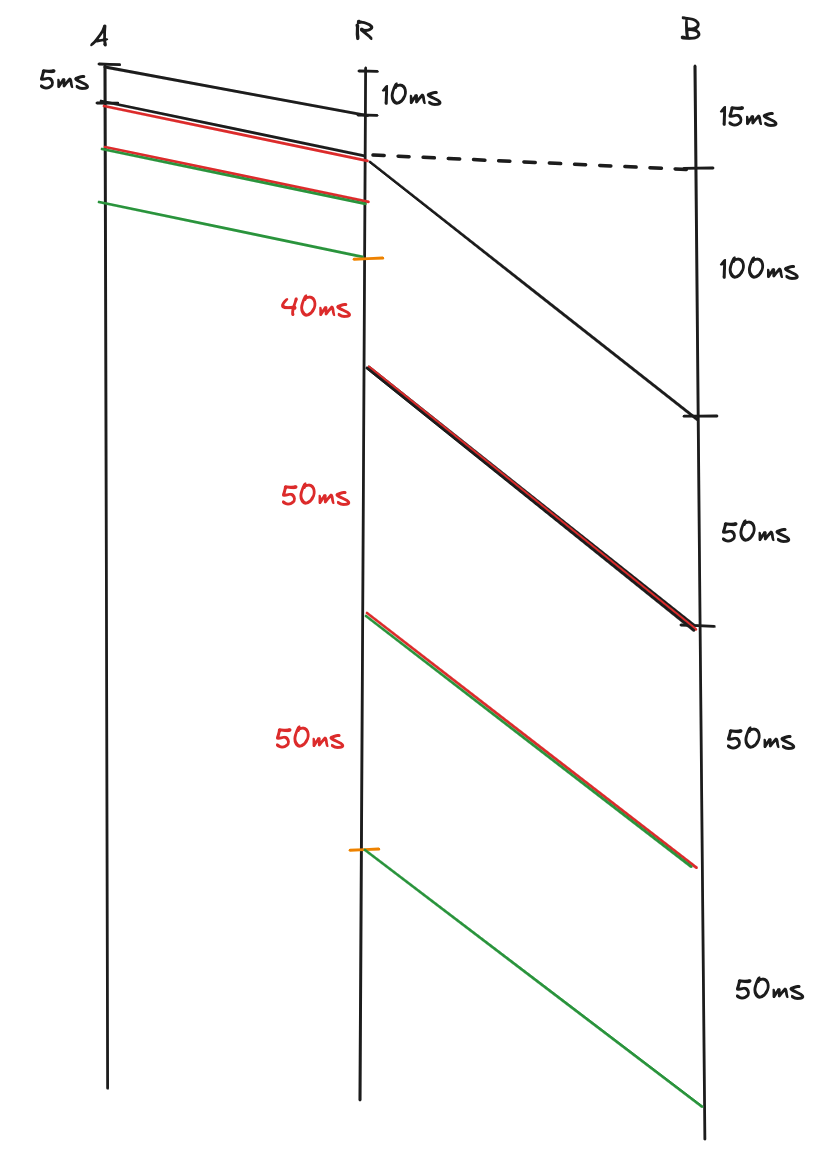
\includegraphics[width=0.6\linewidth]{../src/Q5.jpg}  % 指定图片文件名和宽度
        \caption{Q5}
        \label{fig:5}
    \end{figure}

    \newpage 

    So the queuing delay of the third packet at the router R is $90ms$.
\end{solution}

\newpage
\begin{problem}
    CDMA (10 points)

    Consider 4 stations with the following chip sequences.

    A: (-1 -1 -1 +1 +1 -1 +1 +1)

    B: (-1 -1 +1 -1 +1 +1 +1 -1)

    C: (-1 +1 -1 +1 +1 +1 -1 -1)

    D: (-1 +1 -1 -1 -1 -1 +1 -1)

    The received sequence S = (-1 +1 -3 +1 -1 -3 +1 +1).

    Which station transmitted, and what are the transmitted bits?
\end{problem}

\begin{solution}
    
    $R_A = <S \cdot A>$, $R_B = <S \cdot B>$, and $R_C = <S \cdot C>$

    $$S = (-1 +1 -3 +1 -1 -3 +1 +1)$$
    $$A = (-1 -1 -1 +1 +1 -1 +1 +1)$$
    $$B = (-1 -1 +1 -1 +1 +1 +1 -1)$$
    $$C = (-1 +1 -1 +1 +1 +1 -1 -1)$$
    $$D = (-1 +1 -1 -1 -1 -1 +1 -1)$$

    $$
    <S \cdot A> = \frac{1-1+3+1-1+3+1+1}{8} = 1
    $$

    So A transmitted 1.

    $$
    <S \cdot B> = \frac{1-1-3-1-1-3+1-1}{8} = -1
    $$

    So B transmitted 0.

    $$
    <S \cdot C> = \frac{1+1+3+1-1-3-1-1}{8} = 0
    $$

    So C didn't transmitted.

    $$
    <S \cdot D> = \frac{1+1+3-1+1+3+1-1}{8} = 1
    $$
    
    So D transmitted 1.

    % S = aA + bB + cC + dD

    % $$
    % \begin{cases}
    % -1 = -a - b - c - d \\
    % 1 = -a - b + c + d \\
    % -3 = -a + b - c - d \\
    % 1 = a - b + c - d
    % \end{cases}
    % $$
    
    % So $a = 1$, $b=-1$, $c=0$, and $d=1$. A transmitted 1, B transmitted 0, C didn't transmit, and D transmitted 1.
    So the answer is A, B, and D transmitted, C didn't transmit. A transmitted 1, B transmitted 0, and D transmitted 1.
\end{solution}


\begin{problem}
    Hamming Distance (10 points)

    What is the Hamming distance of the horizontal-vertical parity check code for the $7 \times 7$
    block we discussed in class? Show correctness of your answer by considering the detection
    and correction capability of this coding scheme.
\end{problem}

\begin{solution}

    The Hamming distance of the horizontal-vertical parity check code for the $7 \times 7$ block is 4. 
    beacuse we just need 4 single-bit errors, which is the minimum number required to convert one codeword into another.

    I only found the 5x7 block on the ppt, so I randomly added two rows.
    \begin{figure}[H]
        \centering
        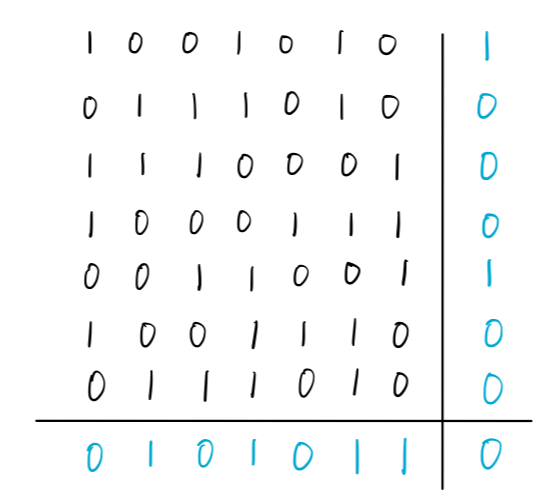
\includegraphics[width=0.6\linewidth]{../src/Q7-1.jpg}  % 指定图片文件名和宽度
        \label{fig:7_1}
    \end{figure}

    The reasons are as follows:

    1. If change 1 bit in the $7 \times 7$, the horizontal parity bit in the corresponding row and the vertical parity bit
    in the corresponding column will be changed. The bit in the lower right corner of the block is also changed. So 4 bits are changed to get another codeword.

    2. If change 2 bits in the $7 \times 7$, If these two bits are in the same row or the same column, only the horizontal parity bit 
    or the vertical parity bit will be changed. In this situation, 4 bits are changed to get another codeword.
    If these two bits are neither in the same row nor in the same column, both the horizontal parity bit and the vertical parity bit will be changed.
    In this situation, 6 bits are changed to get another codeword. So This means at least 3 bits are changed to get another codeword.

    3. If change 3 or 4 bits, the result is as shown below. The image only shows the situation where the bits change the least for changing 3 or 4 bits.

    \begin{figure}[H]
        \centering
        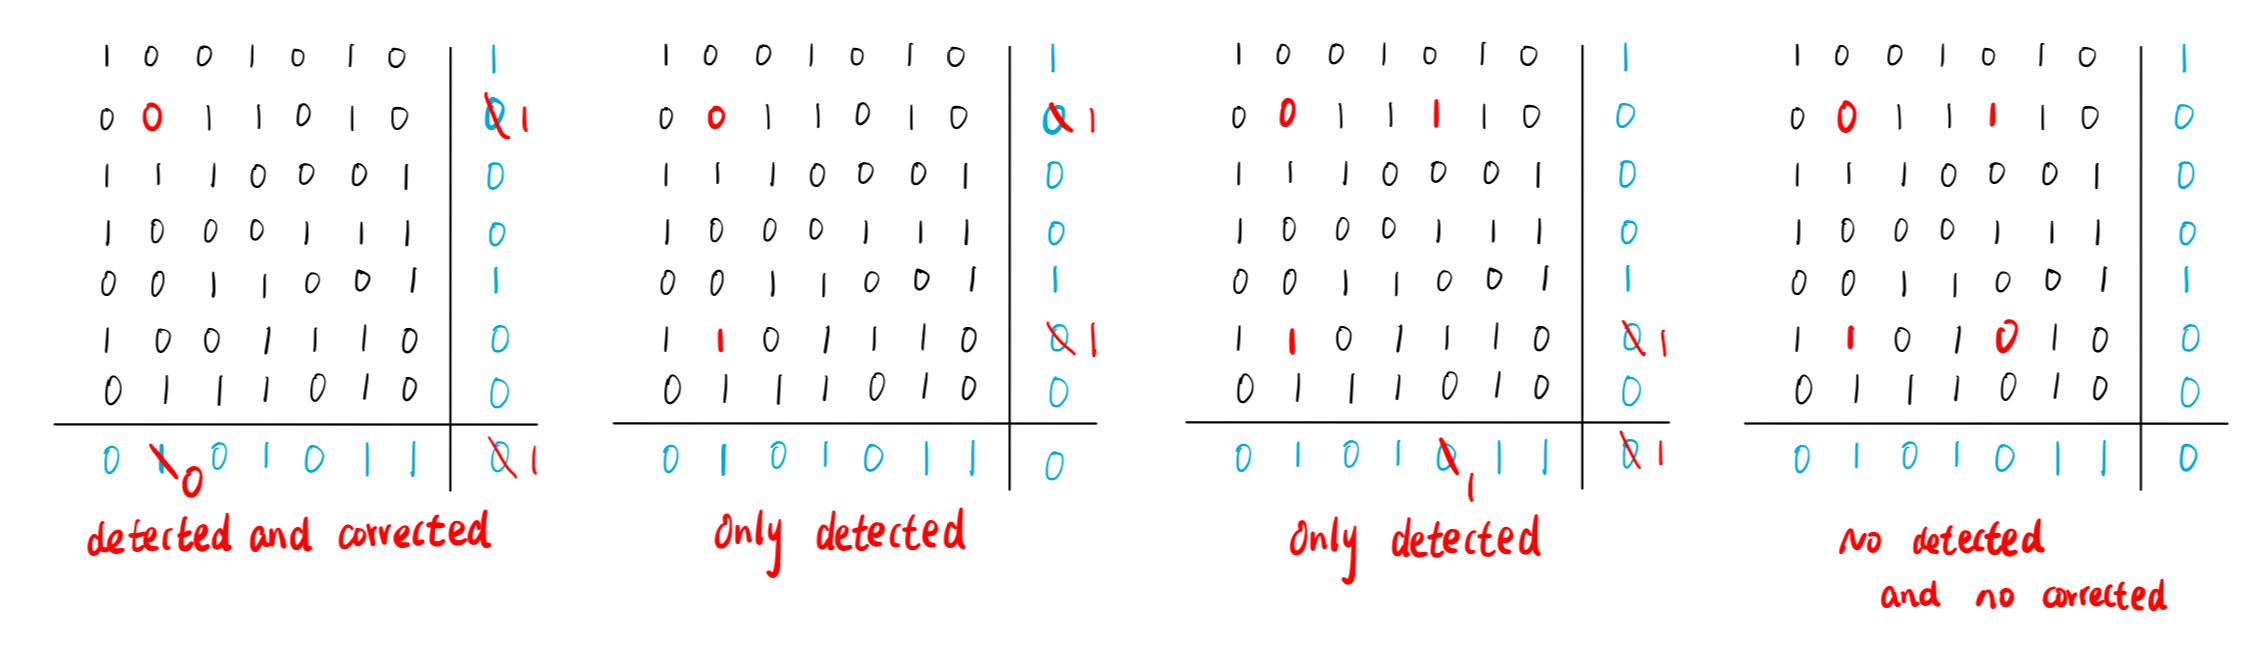
\includegraphics[width=0.9\linewidth]{../src/Q7-2.jpg}  % 指定图片文件名和宽度
        \label{fig:7_2}
    \end{figure}

    4. If change more bits in the $7 \times 7$, we need to change more than 4 bits to get another codeword.

    So, the Hamming distance of the horizontal-vertical parity check code for the $7 \times 7$ block is 4. 
    To show correctness of my answer, I show some examples in the image. To detect $d$ errors, code distance must be $\geq d + 1$; To correct $d$ errors, code distance must be $\geq 2d + 1$ 
    Because the Hamming distance is 4, it can detect 3 bits or correct 1 bits. When changing 4 bits, errors may not be detected. This corresponds to my answer.
\end{solution}


\begin{problem}
    Hamming Code (10 points)

    A 9-bit (m=9) message with binary value 100101011 is to be encoded using a even-parity    Hamming code.

    a) How many check bits are needed?

    b) What is the encoded Hamming codeword. Show your steps.    
\end{problem}

\begin{solution}

    a) $m + r + 1 \leq 2^r$, and $m=9$, so $r_{min}=4$, so 4 check bits are needed.

    b) The insert position of the check bits are 1, 2, 4, and 8. 
    \begin{figure}[H]
        \centering
        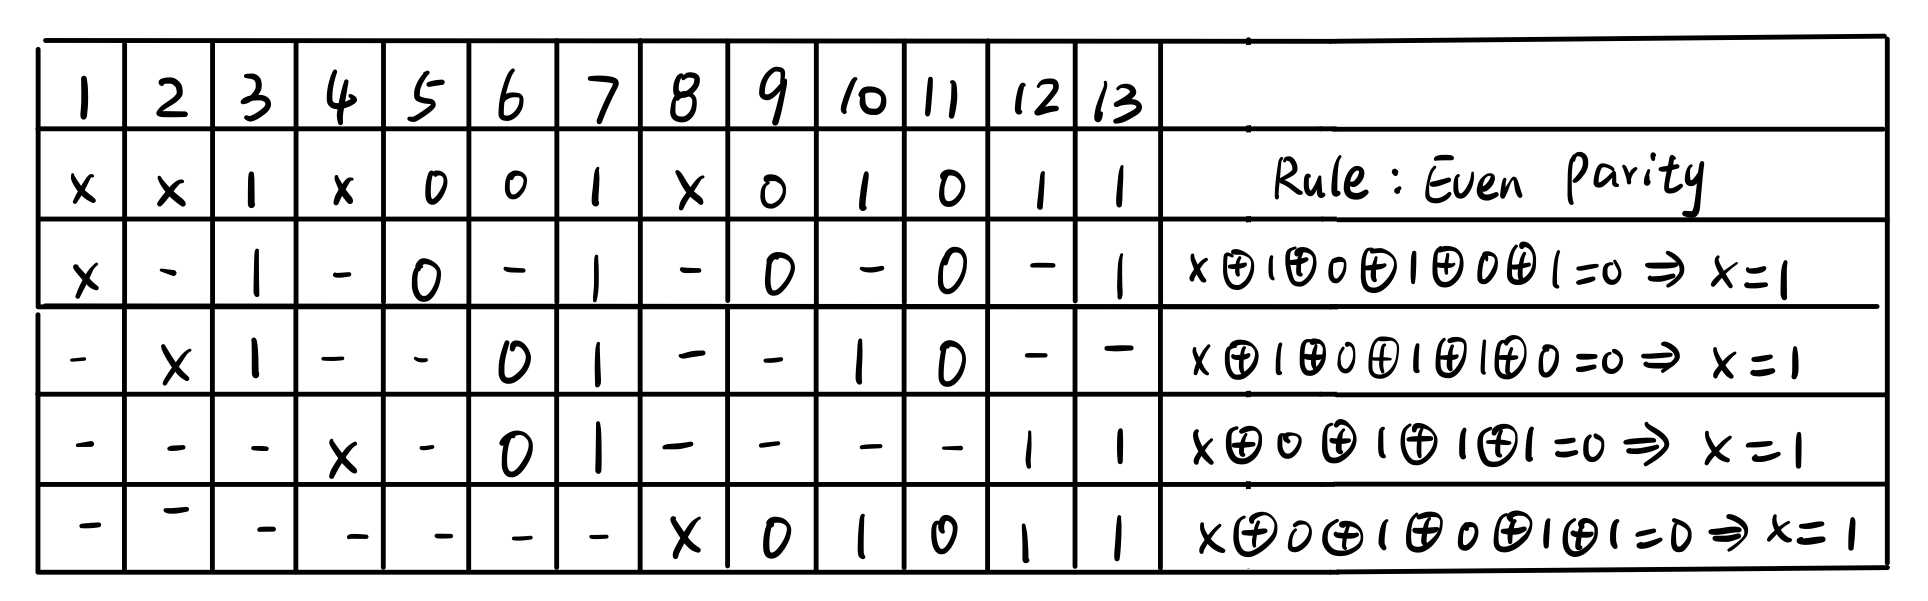
\includegraphics[width=0.6\linewidth]{../src/Q8.jpg}  % 指定图片文件名和宽度
        \caption{Q8}
        \label{fig:Q8}
    \end{figure}

    So, the encoder Hamming codeword is 1111001101011.
\end{solution}

\newpage

\begin{problem}
    CRC (15 points)

    Data stream 10010011101 is to be encoded using the standard CRC method. The generator
    polynomial is $G(x) = x^3 + 1$.

    a) What is the bit string T(x) that is to be transmitted?

    b) Suppose the first three bits from the left are inverted/flipped during the transmission.
    Can the errors be detected? Show your steps. 
\end{problem}

\begin{solution}
    
    a)
    $M = 10010011101$, and $G(x) = x^3 + 1$, so $r=3$ and $k=11$

    $$
    M(x) = x^{10} + x^7 + x^4 + x^3 + x^2 + 1
    $$
    $$
    r(x) = \textit{Remainder} ~[\frac{M(x) \cdot x^r}{G(x)}]
    $$

    \begin{figure}[h]
        \centering
        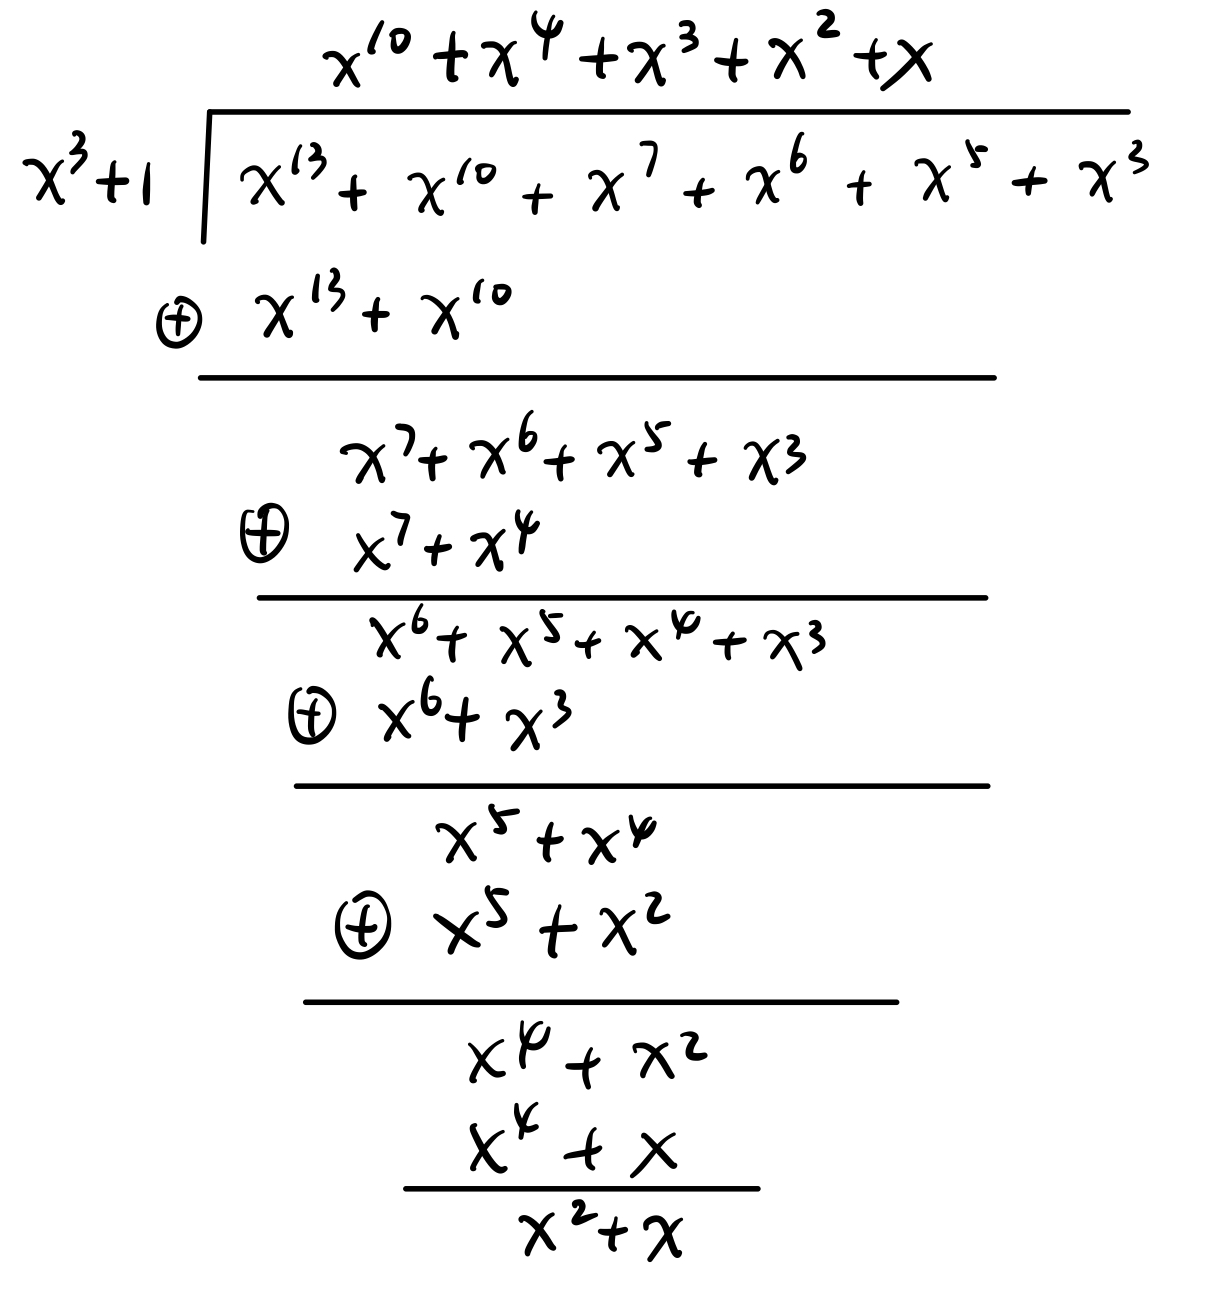
\includegraphics[width=0.4\linewidth]{../src/Q9-1.jpg}  % 指定图片文件名和宽度
        \caption{Q9-1}
        \label{fig:Q9-1}
    \end{figure}

    So, $r(x) = x^2 + x$.
    $$
    T(x) = M(x) \cdot x^r + r(x) = x^{13} + x^{10} + x^7 + x^6 + x^5 + x^3 + x^2 + x
    $$
    
    The bit string $T(X)$ is 10010011101110.
    
    b) 
    The error bit string is 01110011101110.

    \begin{figure}[H]
        \centering
        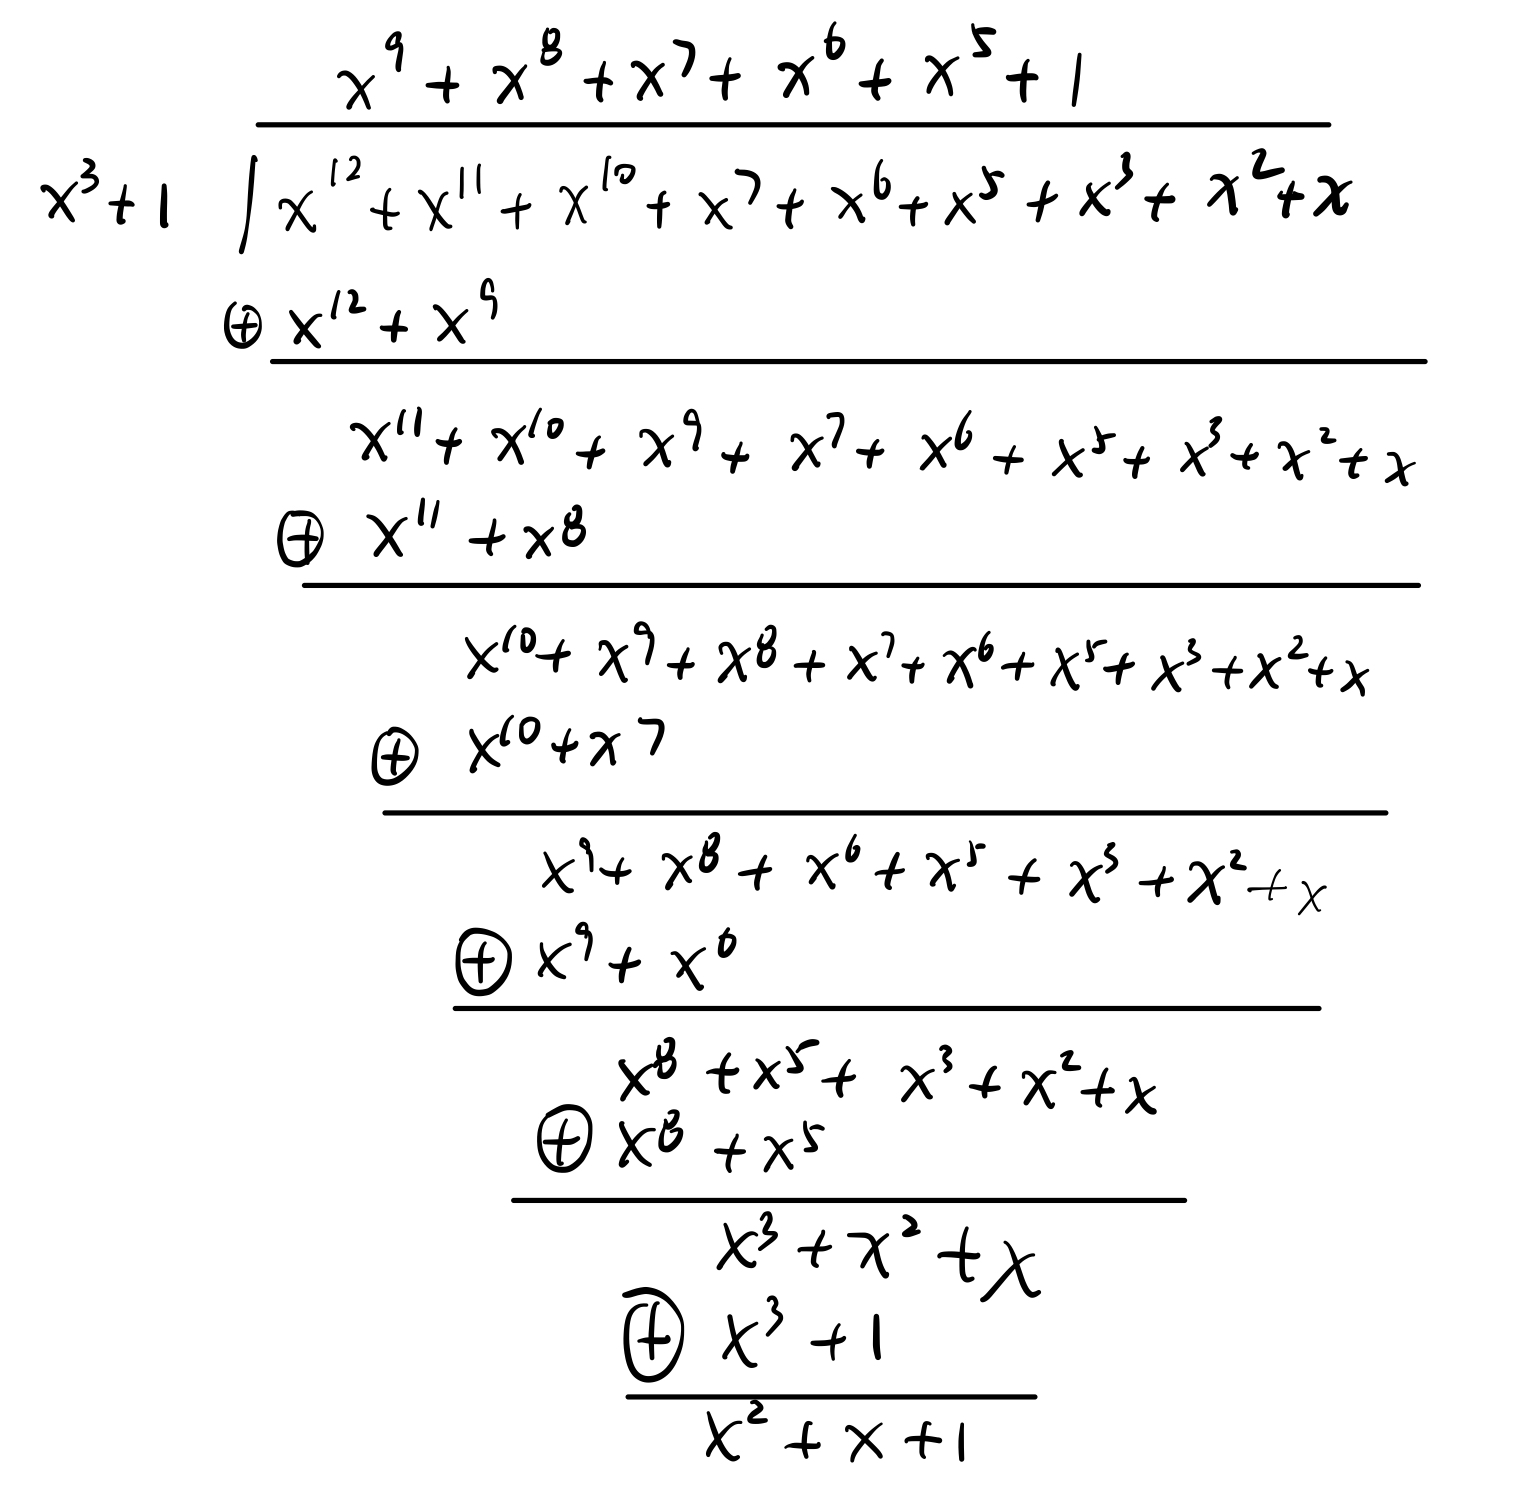
\includegraphics[width=0.4\linewidth]{../src/Q9-2.jpg}  % 指定图片文件名和宽度
        \caption{Q9-2}
        \label{fig:Q9-2}
    \end{figure}

    The remainder is $x^2 + x + 1 \neq 0$, so the errors can be detected.
\end{solution}
\end{document}